\part{Calculus}
\frame{\partpage}

\begin{frame}{Isaac Newton (1643-1727)}
	\begin{columns}
		\begin{column}{0.2\textwidth}
			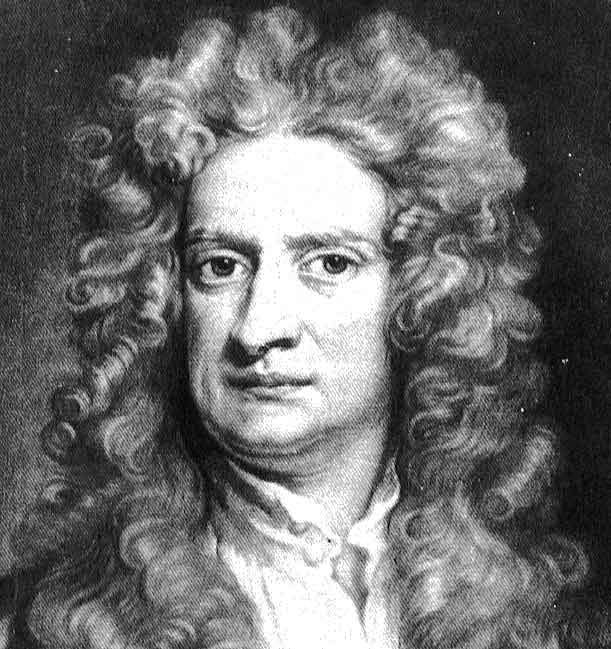
\includegraphics[width=\textwidth]{isaac_newton}
		\end{column}
		\begin{column}{0.78\textwidth}
			\begin{itemize}
				\pause\item Invented \textbf{calculus}
					\begin{itemize}
						\pause\item Study of \textbf{rates of change}
					\end{itemize}
				\pause\item Developed \textbf{laws of motion}
					\begin{itemize}
						\pause\item ``The'' laws of motion until 20th Century (Einstein's theory of relativity, quantum mechanics)
						\pause\item Still useful for motion of ``everyday'' objects (size above quantum scale, speed much lower than speed of light)
					\end{itemize}
				\pause\item Developed \textbf{laws of gravitation}
					\begin{itemize}
						\pause\item Realised that falling objects and orbiting celestial bodies are governed by the same principles
					\end{itemize}
				\pause\item Many other contributions to mathematics and physics
			\end{itemize}
		\end{column}
	\end{columns}
\end{frame}

\begin{frame}{Rates of change}
	\begin{itemize}
		\pause\item Consider a quantity that \textbf{changes over time}
		\pause\item $\text{Rate of change} = \dfrac{\text{change in quantity}}{\text{change in time}}$
	\end{itemize}
	\pause
	\begin{columns}
		\begin{column}{0.4\textwidth}
			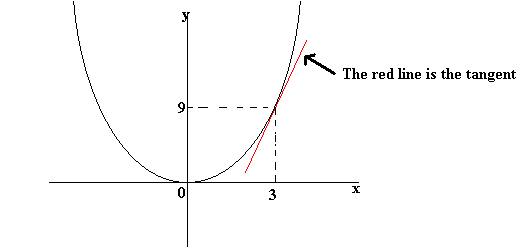
\includegraphics[width=\textwidth]{gradient}
		\end{column}
		\begin{column}{0.58\textwidth}
			Same as the \textbf{gradient} of a graph (from GCSE maths):
			$$\text{gradient} = \dfrac{\text{change in } y}{\text{change in } x}$$
		\end{column}
	\end{columns}
	\begin{itemize}
		\pause\item The \textbf{derivative} of a quantity $x$ with respect to time $t$ is \textbf{the rate of change}
			of $x$ with respect to $t$
		\pause\item Denoted $\dfrac{dx}{dt}$
		\pause\item The mathematical process of finding $\dfrac{dx}{dt}$ given $x$ is called \textbf{differentiation}
	\end{itemize}
\end{frame}

\begin{frame}{Derivatives -- example}
	\begin{itemize}
		\pause\item A car is driving along a straight road at a constant speed
		\pause\item In half an hour, it covers a distance of 20 miles
		\pause\item Its average speed is $\dfrac{20 \text{ miles}}{0.5 \text{ hours}} = 40 \text{ miles per hour}$
		\pause\item In other words...
			\begin{itemize}
				\pause\item \textbf{Distance travelled} is a quantity varying with time
				\pause\item We call the rate of change of this quantity \textbf{speed}
				\pause\item If $x$ is distance travelled and $t$ is time, then we have
					$$\dfrac{dx}{dt} = \dfrac{20}{0.5} = 40$$
			\end{itemize}
	\end{itemize}
\end{frame}

\begin{frame}{Integration}
	\begin{itemize}
		\pause\item Given $\dfrac{dx}{dt}$, find $x$
		\pause\item $x$ is the \textbf{integral} of $\dfrac{dx}{dt}$
		\pause\item The process of finding $x$ is called \textbf{integration}, the opposite of differentiation
		\pause\item We are interested in \textbf{numerical integration}
			\begin{itemize}
				\pause\item I.e.\ integration by computer calculation, not by mathematician with pen and paper...
			\end{itemize}
	\end{itemize}
\end{frame}

\begin{frame}{Euler method}
	\begin{itemize}
		\pause\item If we know values of $x$ and $\frac{dx}{dt}$ at time $t$, we can \textbf{estimate}
			the value of $x$ at time $t+h$
		\pause\item Formula:
			$$ x(t+h) \approx x(t) + h \times \frac{dx}{dt}(t) $$
		\pause\item $\frac{dx}{dt}$ is rate of change, i.e.\ how much $x$ changes by if $t$ changes by $1$
		\pause\item So $h \times \frac{dx}{dt}$ is how much $x$ changes by if $t$ changes by $h$
	\end{itemize}
\end{frame}

\begin{frame}{Euler method}
	\begin{center}
		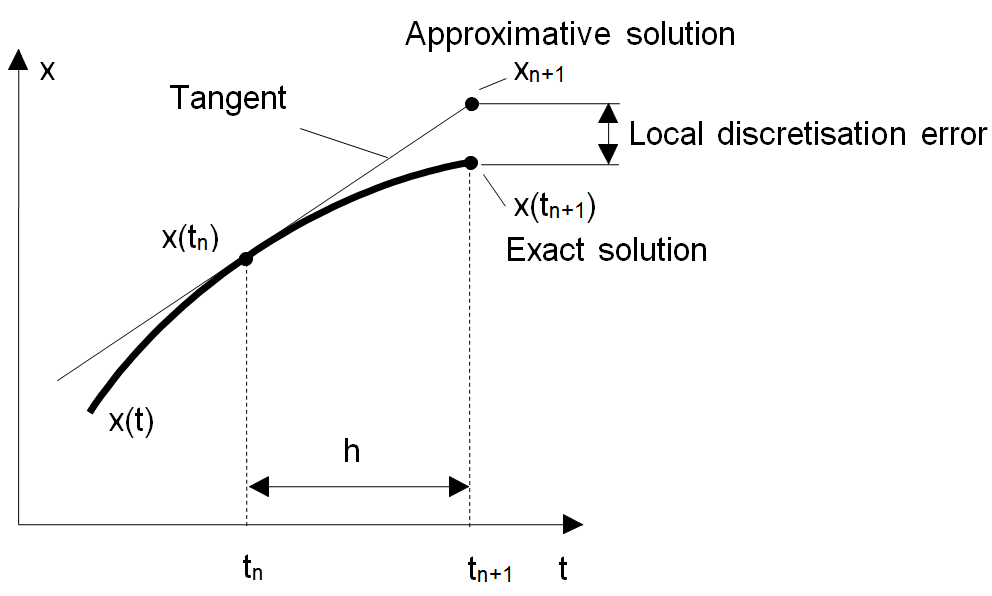
\includegraphics[width=0.6\textwidth]{euler_method}
	\end{center}
	\begin{itemize}
		\pause\item If $\frac{dx}{dt}$ does not change between $t$ and $t+h$, this gives the \textbf{exact} answer;
			otherwise there will be an \textbf{error}
		\pause\item If $h$ is small enough, the error should also be small...
		\pause\item There are more advanced forms of numerical integration which give smaller errors
	\end{itemize}
\end{frame}

\begin{frame}{Calculus with vectors}
	\begin{itemize}
		\pause\item Can talk about rate of change of vectors as well
		\pause\item If $x$ is an $n$-vector, then so is $\frac{dx}{dt}$
		\pause\item Each component of $\frac{dx}{dt}$ is the rate of change of the corresponding component of $x$
	\end{itemize}
\end{frame}
